Program 10:
Develop a LaTeX script to design a simple tree diagram or hierarchical structure
in the document with appropriate labels using the Tikz library
\documentclass{article}
\usepackage{tikz}
\usepackage{fancyhdr}
\pagestyle{fancy}
\fancyhead[l]{Latex,program 10}
\fancyhead[r]{by Sagar}
\fancyfoot[l]{Dept of CSE,GEC,Karwar.}
\fancyfoot[r]{2025-26}
\renewcommand{\headrulewidth}{2pt}
\renewcommand{\footrulewidth}{2pt}
\begin{document}
\begin{figure}[ht]
\centering
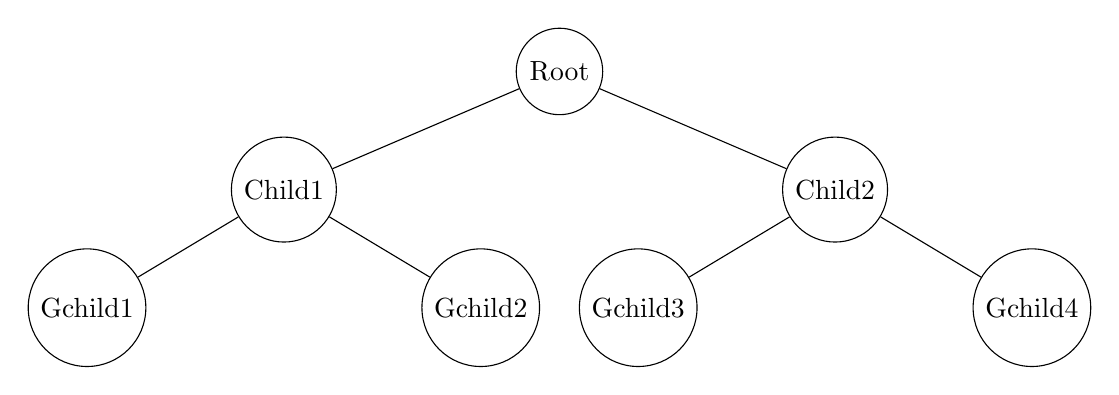
\begin{tikzpicture}[
level 1/.style={sibling distance=7cm},
level 2/.style={sibling distance=5cm},
level 3/.style={sibling distance=25cm},
every node/.style={circle,draw,align=center}
]
\node {Root}
child{node{Child1}
child{node{Gchild1} }
child{node{Gchild2} }
}
child{node{Child2}
child{node{Gchild3} }
child{node{Gchild4} }
};
\end{tikzpicture}
\caption{Hierarchy Diagram}
\label{fig:hierarchy}
\end{figure}
\end{document}
